%\documentclass[twocolumn]{article}
\documentclass[./chem_exercises.tex]{subfiles}
\begin{document}

%\begin{titlepage}
%\maketitle
%\end{titlepage}


%\layout

%\chapter{Syntes av Koppar(II)sulfat}
\textit{\textbf{Inlämningsuppgift Grundläggande\\ begrepp}}

Inlämningsuppgiften består i att besvara följande frågor som listas nedan och besvaras i anslutning till
dessa.
\begin{enumerate}

\item Elektronkonfiguration och kvanttal\\

 Enligt kvantmekaniken får elektoner vistas i olika orbitaler/vågfunktioner/egenfunktioner til Hamilton operatorn som korresponderar till tillåtna energinivåer/egenvärden. Dessa orbitaler definieras av de s.k. kvantalen
$n$, $l$ och $m$. Dessa är relaterade till funktioner som är lösningar till den tidsoberoende Schrödinger ekvationen
för en sfärisk symmetrisk potential.
För att entydigt bestämma elektronens tillstånd tillkommer dock spin som kan vara antingen spin up eller spin ner.
Löser man Schrödinger ekvationen för väteatomen så får man att elektronens energinivåer endast beror
av huvudkvantalet $n$. Energin sägs vara degenerad $n^2$ för väteatomerna med avseende på orbitalerna, men $2n^2$ om spin tas med, medans energinivåerna i fler-elektron atomer
även beror på rörelsemängdsmomentet $l$.\\
Det är alltid så att rörelsemängds momentets $L$ egenvärden bestäms av $l$ där dess värden alltid går från 0 till $n-1$
i heltalssteg oavsett hur komplicerad atomen är och att egenvärdena av  den s.k. z-komponeneten av rörelesmängdsmomentet $L_z$ som kvantifieras med det s.k. magnetiska kvantalet $m$ alltid endast antar värden
från $l$ till $-l$ i heltalsteg även detta oberoende av hur atomen ser ut.
Kvanttalet $l=0$ kallas inom kemin $s$ och då kan $m$ endast anta värdet 0,
vara 0. Denna orbital kan således endast innehålla två elektroner - en med spin upp och en med spin ner där de två måste ha motsatt riktning.
Orbitaler där $l=1$ tillåter endast $m=-1,0,1$ och dessa kallas inom kemin $p_x, p_y, p_z$, vidare då $l=2$ så får $m$ endast anta heltalsvärdena $2,1,0,-1,2$
vilket kemister benämner med olika bokstavsindex relaterat till bokstaven $d$ såsom exempelvis 
$d_x, d_y,d_{x^2+y^2},..$ vilket har som syfte att påminna om vilken symmetri elektrondensiteten har i atomen.
(Källa: Introduction to Quantum Mechanics 2 ed, Griffiths, Chemistry, Chang \& Overby)

\item Elektronegativitet \\

Elektronegativiteten är ett mått på hur starkt en partikel attraherar en elektron. Tydligen är det så att Fluor har högst elektronegativitet
vilket beror på att färre elektroner skärmar den inre positiva kärnan än resten av halogenerna.

\item Gitterenergi \\

\textit{Lattice energy} definieras i boken som den energi som krävs för att separera en en mol av jonerna ingående i en kristallstruktur till fria gasjoner.\\

\item Effektiv kärnladdning\\

Effektiv kärnladdning är den av inre elektroner skärmade kärnladdning som yttre elektroner ``känner'' i en atom.

\item Isotop \\

En isotop av ett grundämne har fler eller färre neutroner än protoner. Exempelvis så är \ch{C^{14}} en isotop av grundämnet kol.

\item Dispersionskrafter \\

Dispersionkrafter sägs enligt boken vara \textit{attraktiva} temporära krafter mellan molekyler i en gas som uppkommer p.g.a.de tillfälliga dipolmoment
hos gasmolekyler som induceras av passerande molekylgranne $A$:s elektronmoln vilken polariserar tillfälligt molekyl $B$ vid nära passage  av $A$ eller vid kollision mellan molekyl $A$
och $B$.
Dessa attraktiva krafter skall vara orsaken till förmågan hos en gas att kondensera.
En illa vald terminologi eftersom dispersion betyder spridning vilket är motsatsen till attraktion.

\item Entalpi\\

Entalpi är ett mått på energi per mängdenhet eller per massenhet och har därför typiskt storheten J/mol eller J/kg.
Vattnets smältentalpi är t.ex. ca 335 kJ \textit {per} kg.

\item Entropi \\

De förklaringar som ges för begreppet Entropi skiljer sig inte från vad man hittar i populärvetenskaplig litteratur vilket säger
någonting om hur pass abstrakt och svårbegripligt det är.
Det sägs vara ett mått på ett systems oordning.
Det sägs, att eftersom en kristallstruktur visar ett högt mått av 
ordning, så kan det därför sägas ha låg entropi, medan en homogen blandning har hög entropi. Enheten för inte intuitivt förståbar
-Joule per Kelvin.
Rent formellt så definieras entropi genom en differens, entropiändring mellan två punkter i en process $\Delta S = S_2-S_1$ som
beräknas genom att ta integralen av infinitesimala ändringar i tillförd/bortförd energi $dQ$ dividerat med temperaturen
T i Kelvin längs en väg(kurvintegralen) mellan två tillstånd i processen, här benämnt $(1)$ och $(2)$\footnotetext[1]{Energiteknik A, Henrik Alvarez}
\begin{flalign*}
\Delta S &=\int \frac{dQ}{T}
\end{flalign*}
Vad betyder detta? Antag att effekten $W$ tillförs en process om 1 J/s under 10 sekunder. För varje 1 sekund $\Delta t$
så tillförs $\Delta Q_i = \Delta W\cdot\Delta t$ och temperaturen $T_i$ noteras i slutet av intervallet
Ändringen i entropi $\Delta S_i$ vid tidpunkterna $t_i$ dvs. $t_1$ till $t_{10}$ är enligt definitionen för
entropiändring
\begin{flalign*}
\Delta S_1 &= \frac{\Delta Q_1}{T_1}\\
\Delta S_2 &= \frac{\Delta Q_1}{T_1}+\frac{\Delta Q_2}{T_2}\\
\Delta S_3 &= \frac{\Delta Q_1}{T_1}+\frac{\Delta Q_2}{T_2}+\frac{\Delta Q_3}{T_3}\\
\vdots\\
\Delta S_{tot} &=\frac{\Delta Q_1}{T_1}+\frac{\Delta Q_2}{T_2}+\frac{\Delta Q_3}{T_3}+..+\frac{\Delta Q_{10}}{T_{10}}\\
\end{flalign*}
Förhållandet mellan täljare och nämnare bestämmer om entropiökningen är stor eller liten.
Tydligen är det så (varför?) att om sluttemperaturen är liten i förhållande till täljaren så
är entropiökningen stor dvs. gasmolekylerna är mer oordnade än om sluttemperaturen för samma
tillförda mängd energi hade varit större.Inte undra på att läroboksförfattare överlämnar beviset med ``varm hand''
till läsaren :-(\\

\item Isobar- , isokor- och isoterm process 

Dessa är termer som används vid studier av gaser. Tillståndet hos en gas definieras entydigt av variablerna tryck, volym, massa, specifik gaskonstant
och temperatur\\
$(p,V,m,R,T)$. Antag att vi har en uppställningen med en gas i en behållare och att vi med en kolv och en brännare kan variera tryck, volym
och temperatur.\\

 Under en \textit{isobar process} så hålls trycket konstant\footnotemark[1]. De variabler som måste variera då
för att åstakomma detta är temperatur $T$ och volym $V$ vilket inses om man ställer upp allmänna gaslagen
\begin{flalign*}
p_1&=\frac{mRT_1}{V_1}\\
p_2&=\frac{mRT_2}{V_2}\\
p_1&=p_2 \implies\\
\frac{\cancel{mR}T_1}{V_1}&=\frac{\cancel{mR}T_2}{V_2}\\
\end{flalign*}
Om vi ökar volymen så måste vi slå på brännaren och värma för att kvoterna $T_1/V_1$ och $T_2/V_2$ skall vara lika.
Om vi trycker in kolven och minskar volymen måste värme bortföras för att trycket ska kunna vara konstant
I ett $p-V$ diagram blir detta en rak horisontell linje.\\
För att öka temperaturen $\Delta T$ så krävs värmetillförsel $\Delta Q$ av storleken
\begin{flalign*}
\Delta Q=mc_p\Delta T
\end{flalign*}
där $c_p$ är den specifika värmekapaciviteten vid konstant tryck och är olika för olika gaser.\\

Under en \textit{iskor process} så hålls volymen konstant\footnotemark[1]. Trycket ökar då vi tillför värme och minskar då värme
bortförs.
\begin{flalign*}
\frac{p_1}{T_1}&=\frac{p_2}{T_2}
\end{flalign*}
För att öka temperaturen $\Delta T$ så krävs värmetillförsel $\Delta Q$ av storleken
\begin{flalign*}
\Delta Q=mc_v\Delta T
\end{flalign*}
där $c_v$ är den specifika värmekapaciviteten vid konstant volym och är olika för olika gaser.\\

Under en \textit{isoterm process} hålls temperaturen konstant\footnotemark[1]. Kompression under konstant temperatur betyder att värme
måste bortföras $\Delta Q < 0$. Expansion under konstant temperatur innebär att värme måste tillföras
$\Delta Q >0 $
\begin{flalign*}
p_1V_1&=p_2V_2
\end{flalign*}

\item Bandteori \\

Bandteori är påståendet att elektroner i halvledare och metaller rör sig i tillåtna energinivåer som 
bildar energiband där energin $E$ har en viss tillåten bredd $\Delta E$ som uppkommer av att delokaliserade
valenselektroner färdas i överlappande molekylära orbitaler över metallen halvledaren. Detta beror på att
en elektron kolliderar  med andra elektroner och interagerar med jonernas positioner i kristallen. Till detta
kommer gittersvängningar. Detta tillsammans gör att elektronerna rör sig inom energiband och inte mellan
energinivåer såsom i en atom eller en molekyl. Förmodligen finns även breddning av energispektra
hos en molekyl som vibrerar i olika moder, men det är spekulation.

\item Ligandteori

Ligandteori är en teori som söker förklara elektron energistrukturen hos molekyler vars centralatom tillhör
övergångs-elemententen.
Det verkar krångligt men tydligen sker det konstigheter relaterade till d-orbitalen hos central atomen då denna tillhör
övergångs-elementen och ligandfält teorin söker förklara energinivåer som den tidigare kristallfält teorin inte kunde.
Det ser ut som att det går ut på att man ska ansätta en linjär kombination av molekylorbitaler $\sigma$- och $\pi$-orbitalerav liganderna
(som i sig själva är linjärkombinationer av atomorbitaler) och bilda s.k. ligandorbitaler.
sådant att de överlappar med atomorbitalerna hos centralatomen. Dessa ligandorbitaler
ska kombineras så att de överlappar med centralatomens valensorbitaler vilket torde betyda att de ska ha samma symmetri som som molekylen.\footnote[2]{\url{https://chem.libretexts.org/Bookshelves/Inorganic_Chemistry/Supplemental_Modules_and_Websites_(Inorganic_Chemistry)/Ligand_Field_Theory/Ligand_Field_Theory_Fundamentals}}
\footnote[3]{\url{https://chem.libretexts.org/Bookshelves/Inorganic_Chemistry/Map\%3A_Inorganic_Chemistry_(Miessler_Fischer_Tarr)/10\%3A_Coordination_Chemistry_II_-_Bonding/10.03\%3A_Ligand_Field_Theory/10.3.01\%3A__Ligand_Field_Theory_-_Molecular_Orbitals_for_an_Octahedral_Complex}}
Ansätter man sådana vågfunktioner när man löser Schrödinger ekvationen så fås korrekta energier såsom egenvärden.






\end{enumerate}

%\vfill\null
%\clearpage
%\columnbreak
%\newpage



%\underbrace{}

% \hspace{1em}

%\begin{enumerate}[label=(\alph*)]
%\end{enumerate}

%$$
%  A = 
%  \begin{bmatrix}
%    1 & 0  & 2i\\
%    2i & 0 &  -4\\
%    -i &  0 & -2i\\
%  \end{bmatrix}
%$$

%\begin{flalign*}
%  A = 
%  \begin{bmatrix}
%    1 & 0  & 2i\\
%    2i & 0 &  -4\\
%    -i &  0 & -2i\\
%  \end{bmatrix}
%\end{flalign*}


%\begin{flalign*}
%\psi(x) = \begin{cases} Ae^{ikx}+Be^{-ikx} &\ \  x<-a \\
%                        Ce^{\kappa x}+De^{-\kappa x} &\ \ -a < x < a\\
%						Fe^{ikx} & \ \ x>a
%       \end{cases}
%\end{flalign*}

%\begin{figure}[H]
%  \includegraphics[width=\linewidth]{odd_finite.eps}
%  \caption{$z_0=0.1\pi,0.5\pi, 3\pi,7\pi$}
%  \label{fig4}
%\end{figure}
\end{document}









\leavevmode\marginpar{
\centering
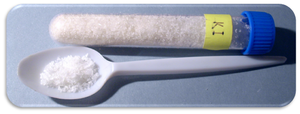
\includegraphics[scale=0.4]{KI.png}
\captionof{figure}{Kaliumjodid, \ch{KI}}
\label{fig6}
}





\vfill\null
\clearpage
\columnbreak
\newpage










                                     
                                     



